\clearpage
%%=========================================
\section{LPE - Hall, FTIR, SIMS}

\todo{Have to add SIMS to both Method chapter and Experimental details chapter (Why is SIMS used?).} \Ac{sims} profiles of \ce{Na}, \ce{Al}, \ce{Si}, \ce{K}, \ce{Fe}, \ce{Ni}, \ce{Cu}, and \ce{Pb} from two different locations on sample LPE422 are shown in Fig.~\ref{fig:sims_lpe422}. The measurements show that \ce{Na}, \ce{Al}, \ce{Si}, \ce{K}, and \ce{Fe} are found at the interface between the substrate and the grown layer as peak concentrations. \ce{Ni}, \ce{Cu}, and \ce{Pb}, with detection limits of \SI{1e14}{}, \SI{2e14}{}, and \SI{2e13}{\atom\centi\metre^{-3}} respectively, were not detected throughout the \ce{HgCdTe} film and \ce{CdZnTe} substrate.

\ce{Si} and \ce{K} were detected in neither the \ce{HgCdTe} film nor in the \ce{CdZnTe} substrate. \todo{Where does the Si and K come from?}

\ce{Na} and \ce{Al} were not detected in the \ce{HgCdTe} film, but were detected in the \ce{CdZnTe} substrate. \todo{Why doesn't Al diffuse into the layer? Why is there a minimum in the Na concentration right after the peak before it grows into the substrate?}

\ce{Fe} was detected throughout both the \ce{HgCdTe} layer and the \ce{CdZnTe} substrate. Higher \ce{Fe} concentration was detected with a peak \ce{Fe} concentration likely at the interface of \ce{HgCdTe} and \ce{CdZnTe}. This higher concentration of \ce{Fe} was found between a depth of \SI{\sim 13}{\micro\metre} and \SI{23}{\micro\metre} for the first measurement, and between a depth of \SI{\sim 16}{\micro\metre} and \SI{23}{\micro\metre} for the second measurement. The \ce{Fe} peak stands out \todo{... explanation of the different shapes: Why does the \ce{Fe} concentration have a wide concentration peak? And why is it in both the substrate and the layer?} \todo{Group 1A and 1B diffuse faster than other?}

%\todo{Cadmium is cation, and tellurium is anion.}

\todo{\Ac{ftir}}

\todo{Hall}

\begin{figure}[htbp]
    \centering
    \subfigure[W3]{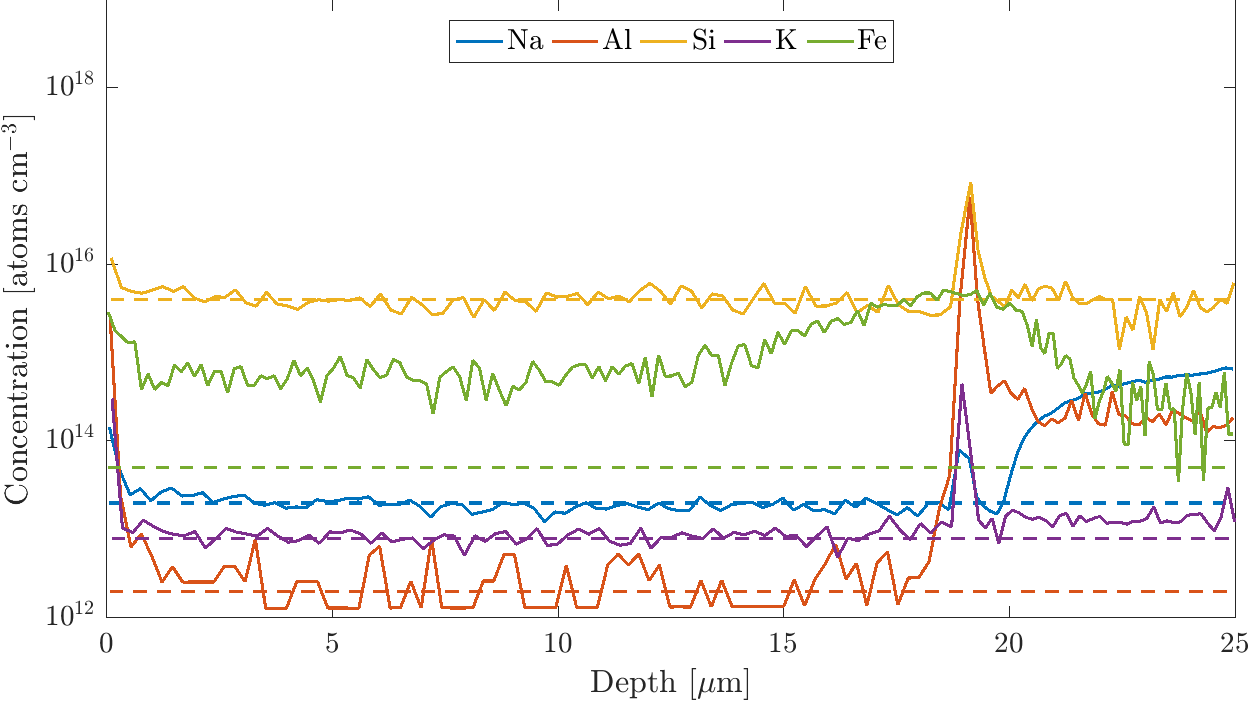
\includegraphics[width=0.90\linewidth]{sims_lpe422_w3.png}}
    %\quad
    \subfigure[W4]{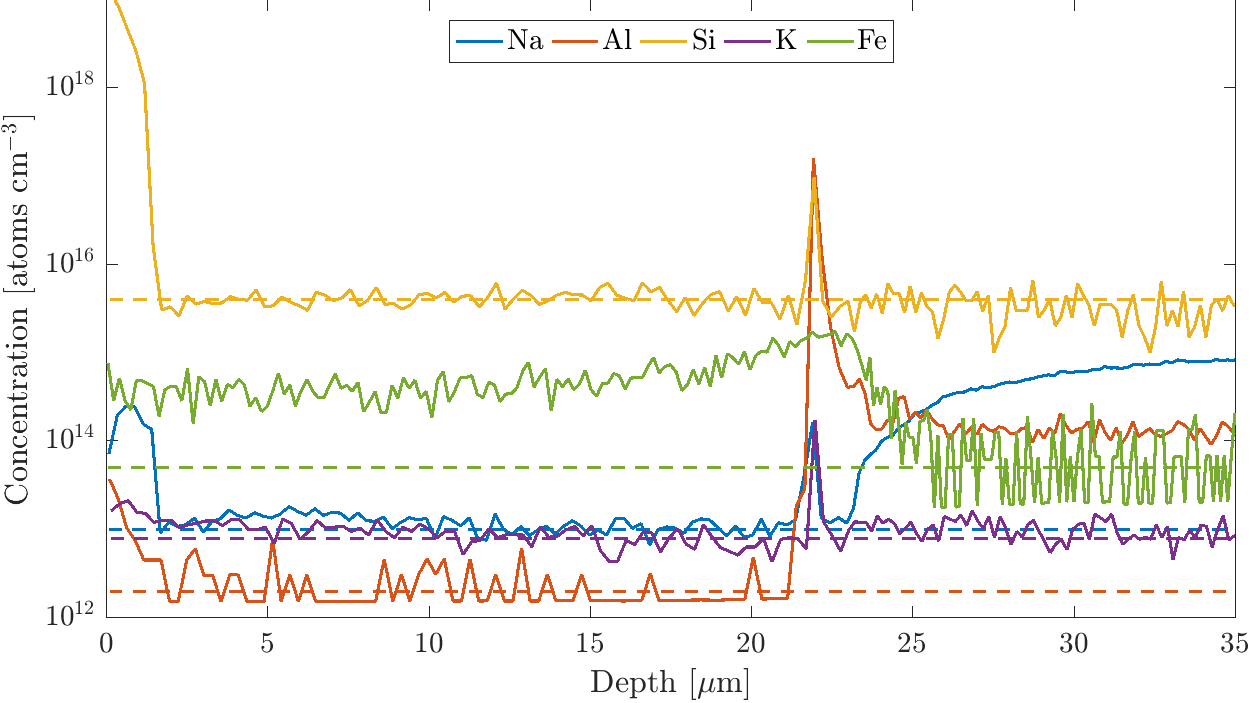
\includegraphics[width=0.90\linewidth]{sims_lpe422_w4.png}}
    \caption[\Ac{sims} profiles from sample LPE422.]{\Ac{sims} profiles of \ce{Na}, \ce{Al}, \ce{Si}, \ce{K}, and \ce{Fe} atom concentration in sample LPE422. These are the profiles for the epitaxial \ce{HgCdTe} layer grown by \ac{lpe} on a (111)B \ce{CdZnTe} substrate from vendor B. \ce{Ni}, \ce{Cu}, and \ce{Pb}, with detection limits of \SI{1e14}{}, \SI{2e14}{}, and \SI{2e13}{\atom\centi\metre^{-3}} respectively, were not detected. The solid line is the concentration of an element, while the dashed line is the detection limit of that element.}
    \label{fig:sims_lpe422}
\end{figure}
%%=========================================

\todo{LPE smelte størkner tidligere ved urenheter -> krystallinske defekter i laget.}